\scanpage{45}
\diagram{\begin{tikzcd}[ampersand replacement=\&,row sep=small,column sep=small]
\&\unsure{\zeta|s|\}}_{14}\arrow[r,dash]\arrow[dl,dash,shift left]\arrow[dl,dash,shift right]\&\zeta_{25}\arrow[dll,dash]\arrow[dr,dash]\&\deleted{\unsure{\zeta_1|\zeta_{15}}}\\
\zeta_{\unsure{35|32|34}}\arrow[dr,dash]\&\&\&\zeta_{16}\arrow[dll,dash,shift left]\arrow[dll,dash,shift right]\\
\&\zeta_{24}\arrow[uur,dash]\&\&
\end{tikzcd}}
\[
\begin{aligned}
 & &\zeta_{14}&\\
 &\zeta_{25}&&\zeta_{26}\\
 &\zeta_{16}&&\zeta_{15}\\
 &&\zeta_{24}&
\end{aligned}
\]
\figure{\begin{tikzpicture}[x=.72cm,y=.72cm]
\draw (-1.6,.05)--(.32,1.12)--(1.12,-.05)--(.30,-1.25)--(-.78,-1.16)--cycle;
\draw (-.78,-1.16)--(-.2,-.44)--(.30,-1.25) (-.8,-1.0)--(-.82,.9) (-.86,1.12)--(.32,1.12) (-.86,1.12)--(-.31,1.75)--(-.5,.86);
\node[left] at (-1.5,.09) {$\unsure{a|x_1}$}; \node[below] at (-1.42,.09) {$\unsure{=}$};
\node[left] at (-.86,1.15) {$\unsure{x|x_2}$};\node[above] at (.32,1.12) {$x_4$}; \node[right] at (.33,1.12) {$=\unsure{t|r|\zeta}$};
\node[right] at (1.06,-.05) {$\deleted{\unsure{x}}x_3=\unsure{s|5|\zeta}$};
\node[above] at (-.2,-.44) {$b$};\node[below] at (.45,-1.25) {$x_5=a$};
\node[below] at (-.82,-1.18) {$\substack{\unsure{x_6}\,-\\\unsure{{}''e|{}=\zeta}}$};\draw (-.8,-1.76) to[bend right=10] (-.69,-2.05);
\end{tikzpicture}}
\[
15\cdot6\cdot4\cdot2\cdot1=720=6!
\]
\[
\begin{aligned}
&\underbrace{\overline{\zeta_{13}}\,\overline{\zeta_{24}}\,\overline{\zeta_{35}}\,\overline{\zeta_{41}}\,\zeta_{52}}\\
&\zeta_{15}\quad\zeta_{32}\quad\zeta_{54}\quad\zeta_{21}\quad\zeta_{\unsure{43|47}}
\end{aligned}
\]
\[
\zeta_{12}\ \unsure{\zeta|\}}
\]
\figure{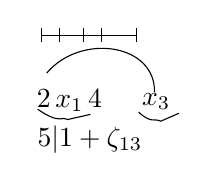
\begin{tikzpicture}[x=.72cm,y=.72cm]
\draw (-.1,1.6)--(1.6,1.6);
\foreach \x in {-.1,.23,.65,.96,1.58}{\draw (\x,1.48)--(\x,1.73);}
\draw (0,.94) .. controls (.6,1.65) and (1.92,1.46) .. (1.9,.6);
\node at (.4,.45) {$\deleted{\unsure{2}}\,x_1\,\deleted{\unsure{4}}$};
\node at (1.93,.44) {$x_3$};
\draw (-.16,.30) .. controls (.25,.02) and (.27,.19) .. (.37,.12) -- (.77,.21);
\draw (1.62,.25) .. controls (1.85,.04) and (1.89,.15) .. (2.01,.09) -- (2.33,.23);
\node at (.76,-.24) {$\unsure{5|1}+\zeta_{13}$};
\end{tikzpicture}}
\figure{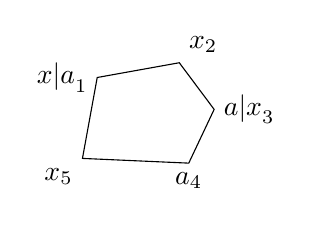
\begin{tikzpicture}[scale=.75]
\draw (-.91,.69)--(.48,.94)--(1.07,.15)--(.64,-.76)--(-1.16,-.68)--cycle;
\node[left] at (-.91,.69) {$\unsure{x|a}_1$};\node[above right] at (.48,.94) {$x_2$};
\node[right] at (1.07,.15) {$\unsure{a|x}_3$};\node[below] at (.64,-.76) {$a_4$};
\node[below left] at (-1.16,-.68) {$x_5$};
\end{tikzpicture}}
\[
\underline{\zeta_{12}}\,\zeta_{34}\,\zeta_{15}\,\underline{\zeta_{23}}\,\zeta_{45}
\qquad 10\,P=720
\]
\[
\deleted{\unsure{46}}\qquad 2\quad2\quad2\quad2\quad2\quad0\qquad P=72
\]
\figure{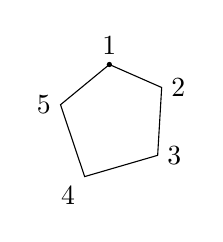
\begin{tikzpicture}[scale=.73]
\draw (0,1)--(.91,.6)--(.84,-.58)--(-.43,-.95)--(-.85,.30)--cycle;
\fill (0,1) circle (1.3pt);
\node[above] at (0,1) {$1$};\node[right] at (.91,.6) {$2$};\node[right] at (.84,-.58) {$3$};\node[below left] at (-.43,-.95) {$4$};\node[left] at (-.85,.30) {$5$};
\end{tikzpicture}}
\[
4!=\qquad
\begin{aligned}P_0&=12\\&=\text{nb \unsure{de|des} struct. pol. sur l'ens à $5$ él}\end{aligned}
\]
\[
\zeta_{i,i+2}\quad\zeta_{j,j+\unsure{2|3}}
\]
\figure{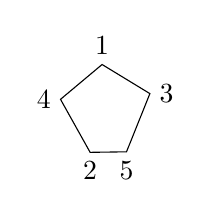
\begin{tikzpicture}[scale=.66]
\draw (0,.96)--(.92,.4)--(.47,-.72)--(-.23,-.73)--(-.8,.29)--cycle;
\node[above] at (0,.96) {$1$};\node[right] at (.92,.4) {$3$};\node[below] at (.47,-.72) {$5$};\node[below] at (-.23,-.73) {$2$};\node[left] at (-.8,.29) {$4$};
\end{tikzpicture}}
% archive sheet number: 44
